\documentclass[12pt, a4paper]{article}
\usepackage[utf8]{inputenc}
\usepackage{tikz}
\usetikzlibrary{shapes.geometric, arrows.meta, positioning, fit, backgrounds, calc}
\usepackage{geometry}
\geometry{a4paper, margin=1in}

\tikzstyle{process} = [rectangle, rounded corners, minimum width=3cm, minimum height=1cm, text centered, draw=black, fill=orange!20, text width=3.5cm, font=\small]
\tikzstyle{database} = [cylinder, shape border rotate=90, aspect=0.25, draw, minimum height=2.5cm, minimum width=3cm, text centered, fill=blue!20, font=\small]
\tikzstyle{client} = [rectangle, rounded corners, minimum width=3cm, minimum height=1cm, text centered, draw=black, fill=green!20, text width=3.5cm, font=\small]
\tikzstyle{external} = [rectangle, rounded corners, minimum width=3cm, minimum height=1cm, text centered, draw=black, fill=gray!20, text width=3.5cm, font=\small]
\tikzstyle{ml} = [rectangle, rounded corners, minimum width=3cm, minimum height=1cm, text centered, draw=black, fill=purple!20, text width=3.5cm, font=\small]
\tikzstyle{arrow} = [thick,->,>=stealth]
\tikzstyle{dashed_arrow} = [thick,dashed,->,>=stealth]
\tikzstyle{labelnode} = [font=\footnotesize, text width=2.5cm, align=center]

\begin{document}

\title{\textbf{Smart Itinerary Planner}\\ \Large System Architecture UML Diagram}
\author{}
\date{}
\maketitle

\vspace{1cm}

\begin{figure}[h]
\centering
\resizebox{\textwidth}{!}{
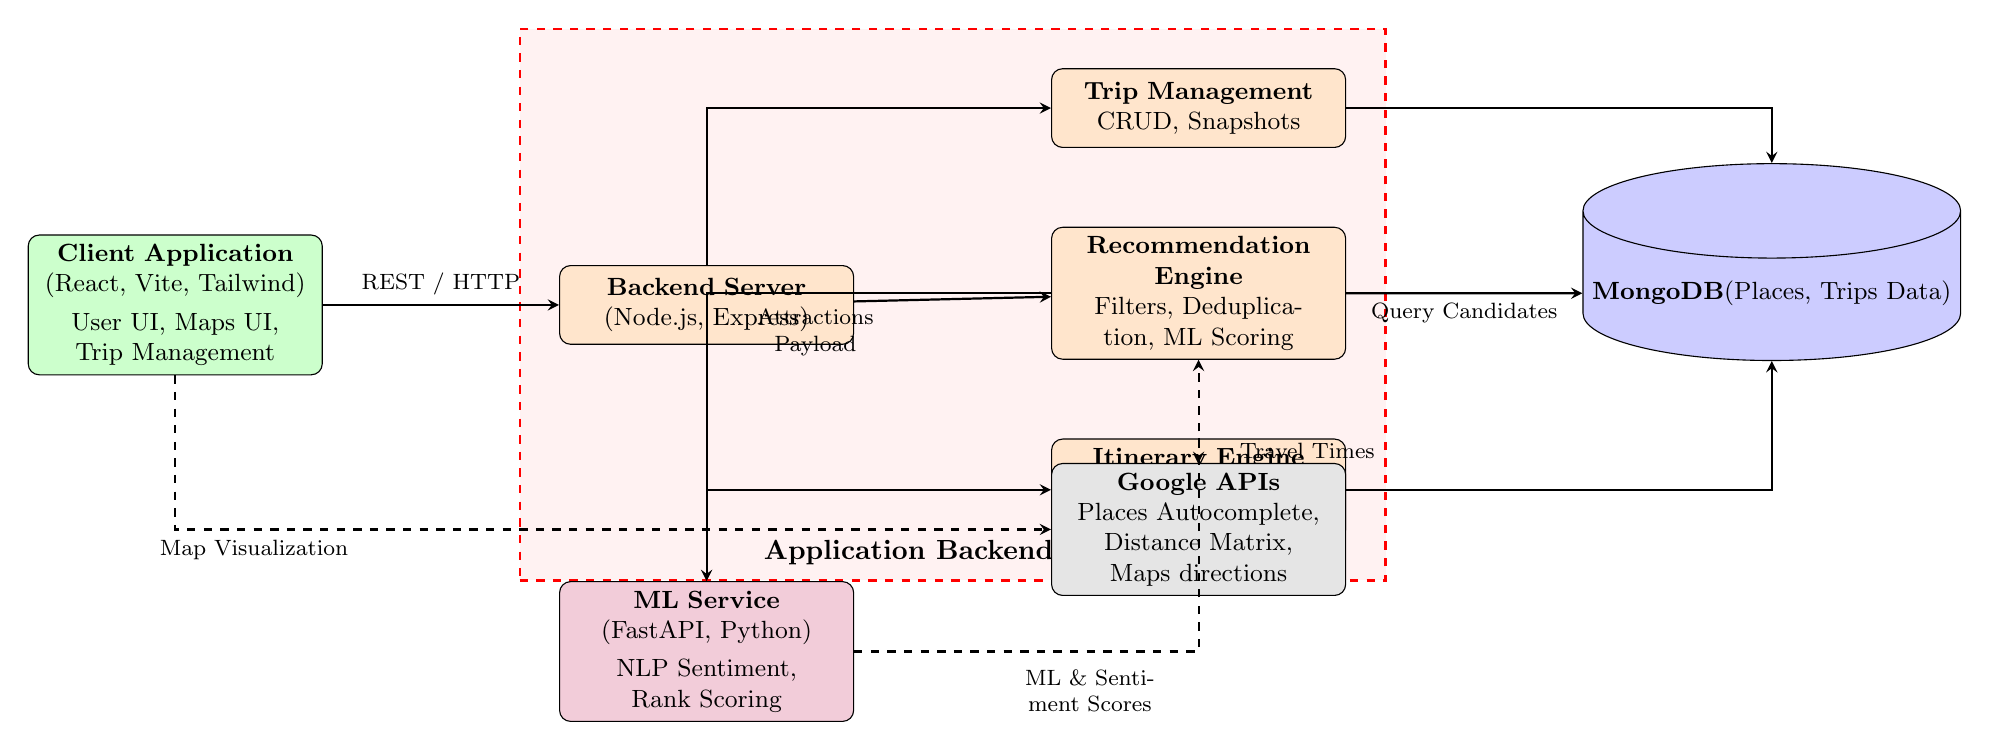
\begin{tikzpicture}[node distance=2.5cm]

% --- Client Layer ---
\node (frontend) [client] {\textbf{Client Application}\\(React, Vite, Tailwind)\\ \vspace{0.1cm} User UI, Maps UI, Trip Management};

% --- Backend Layer ---
\node (gateway) [process, right=3cm of frontend] {\textbf{Backend Server}\\(Node.js, Express)};

\node (trip_mgr) [process, right=2.5cm of gateway, yshift=2.5cm] {\textbf{Trip Management}\\CRUD, Snapshots};
\node (rec_engine) [process, below=1cm of trip_mgr] {\textbf{Recommendation Engine}\\Filters, Deduplication, ML Scoring};
\node (itin_engine) [process, below=1cm of rec_engine] {\textbf{Itinerary Engine}\\Clustering, TSP Routing, Pacing};

% Backend Group Box
\begin{scope}[on background layer]
\node[fit=(gateway)(trip_mgr)(rec_engine)(itin_engine), draw=red, thick, dashed, inner sep=0.5cm, fill=red!5, label={[anchor=south, inner sep=0.2cm]south:\textbf{Application Backend Layer}}] (backend_box) {};
\end{scope}

% --- Database Layer ---
\node (mongodb) [database, right=3cm of rec_engine] {\textbf{MongoDB}\\(Places, Trips Data)};

% --- ML Service ---
\node (ml_service) [ml, below=3cm of gateway] {\textbf{ML Service}\\(FastAPI, Python)\\ \vspace{0.1cm} NLP Sentiment, Rank Scoring};

% --- External Services ---
\node (google_api) [external, below=4cm of trip_mgr] {\textbf{Google APIs}\\ Places Autocomplete, Distance Matrix, Maps directions};

% --- Connections ---
% Client to Backend
\draw [arrow] (frontend) -- node[anchor=south, labelnode] {REST / HTTP} (gateway);

% Gateway to Modules
\draw [arrow] (gateway) |- (trip_mgr);
\draw [arrow] (gateway) -- (rec_engine);
\draw [arrow] (gateway) |- (itin_engine);

% Modules to Database
\draw [arrow] (trip_mgr) -| (mongodb);
\draw [arrow] (rec_engine) -- node[anchor=north, labelnode] {Query Candidates} (mongodb);
\draw [arrow] (itin_engine) -| (mongodb);

% Recommendation Engine to ML Service
\draw [arrow] (rec_engine) -| node[anchor=west, labelnode, yshift=-0.5cm] {Attractions Payload} (ml_service);
\draw [dashed_arrow] (ml_service) -| node[anchor=east, labelnode, yshift=-0.5cm] {ML \& Sentiment Scores} (rec_engine);

% External API Connections
\draw [dashed_arrow] (itin_engine) -- node[anchor=west, labelnode] {Travel Times} (google_api);
\draw [dashed_arrow] (frontend) |- node[anchor=north, labelnode, xshift=1cm] {Map Visualization} (google_api);

\end{tikzpicture}
}
\caption{High-Level Architecture and Data Flow}
\end{figure}

\newpage

\section*{Architecture Components Deep-Dive}

Based on the implemented features of the Smart Itinerary Planner, the system is logically divided into three primary layers.

\subsection*{1. Client Layer}
Built with \textbf{React, Vite, and Tailwind CSS}.
\begin{itemize}
    \item \textbf{Trip Creation \& Management:} Allows users to define destination, days, budget, interests, and starting hotel locations using Google Places Autocomplete.
    \item \textbf{Persisted Snapshots:} Reloads previously generated recommendations and daily itineraries seamlessly without regeneration.
    \item \textbf{Google Maps UI Integration:} Renders real road routes using Google Directions, visualizes custom markers, and synchronizes selection states between the map and itinerary cards.
\end{itemize}

\subsection*{2. Backend Application Layer}
Built with \textbf{Node.js and Express}, interacting with \textbf{MongoDB}.
\begin{itemize}
    \item \textbf{Trip Management:} Handles the domain model for Trips, saving state snapshots of recommendations and routes.
    \item \textbf{Recommendation Engine:}
    \begin{itemize}
        \item \textbf{Candidate Fetch:} Retrieves large batches of highly-rated attractions based on city and popularity.
        \item \textbf{Filtering Pipeline:} Selects based on strict Google Place attraction types, ignoring specific generic types, and validating rating/review thresholds.
        \item \textbf{Interest-Based Sampling:} Blends popularity-driven candidates with user-specific interest matches (e.g., matching "Culture" to museums and historic sites).
        \item \textbf{Scoring:} Fuses internal dynamic metrics (must-see boost, weighted ratings) with the AI scores received from the ML Service.
    \end{itemize}
    \item \textbf{Itinerary Engine:}
    \begin{itemize}
        \item \textbf{Clustering:} Utilizes \texttt{ml-kmeans} to logically group geographic points by trip days.
        \item \textbf{TSP Routing:} Establishes sequential visit chains using minimal travel-time estimations dynamically retrieved from the Google Distance Matrix.
        \item \textbf{Pacing \& Constraints:} Fits places into specific time slots, rigorously respecting destination opening-hours logic, travel times, and inserting meal breaks automatically.
    \end{itemize}
\end{itemize}

\subsection*{3. ML Inference Service}
A lightweight \textbf{FastAPI (Python)} application specifically engineered for ML tasks.
\begin{itemize}
    \item Accepts payloads from the Backend Recommendation Engine containing attraction data and reviews.
    \item Uses pre-trained NLP models to calculate sentiment scores and generic recommendation ranking scores, which dictate over 45\% of the total place ranking weight.
\end{itemize}

\subsection*{4. Database \& External Apis}
\begin{itemize}
    \item \textbf{MongoDB:} Serves as the primary persistence layer holding tens of thousands of enriched city attractions and dynamic user trip information.
    \item \textbf{Google APIs:} Integral to correct UI rendering and intelligent routing (Distance Matrix latency algorithms).
\end{itemize}

\end{document}
